\documentclass[14pt, a4paper]{article}
\usepackage{amsmath}
\usepackage{amssymb}
\usepackage[style=authoryear, backend=biber, maxnames=3]{biblatex} % for the citation, 
\usepackage{hyperref}
\addbibresource{bibentries.bib}
\usepackage{graphicx}
\usepackage[utf8]{inputenc}
\setlength\parindent{0pt}
\renewcommand{\baselinestretch}{1.5} 
\graphicspath{{../../}}



\title{Humboldt-Project 2017-2018:\\ Big Data in Election Forecasting}
\author{Marcel Schliebs\thanks{Zeppelin Universität}\footnotemark[2]}
\date{Research Protocol No. 1 (\textit{Version as of \today})}

\begin{document}
\maketitle

\rule{\linewidth}{0.4pt}
\begin{abstract}
This is the abstract
\end{abstract}
\textbf{Keywords:} asdasd, asd, asd\\
\medskip
\textbf{JEL codes:} asdasd, asd, asd\\
\rule{\linewidth}{0.4pt}


\maketitle

\tableofcontents
\newpage


\section{Introduction}

...\\
...\\
...\\
...\\
...\\
...\\

\section{Gesprächsprotokoll Flo}



\section{Literature \& Theory}

\section{Data Collection}

In order to build a solid basis for later analysis, I have started to build a database of polls, individual-level surveys and micro-level constituency election results data. 
I will hence briefly present the individual sources. 

\subsection{Polls}

\subsubsection{Bundestagswahl - National election}

\subsubsection{Landtagswahlen - State election}


\subsection{Surveys}

\section{Next steps}







\begin{figure}
\caption{A Figure using R}
\centering
\includegraphics[width=0.75\textwidth]{results/figures/a1.jpg}
\end{figure}

\begin{figure}
	\caption{A Figure using R}
	\centering
	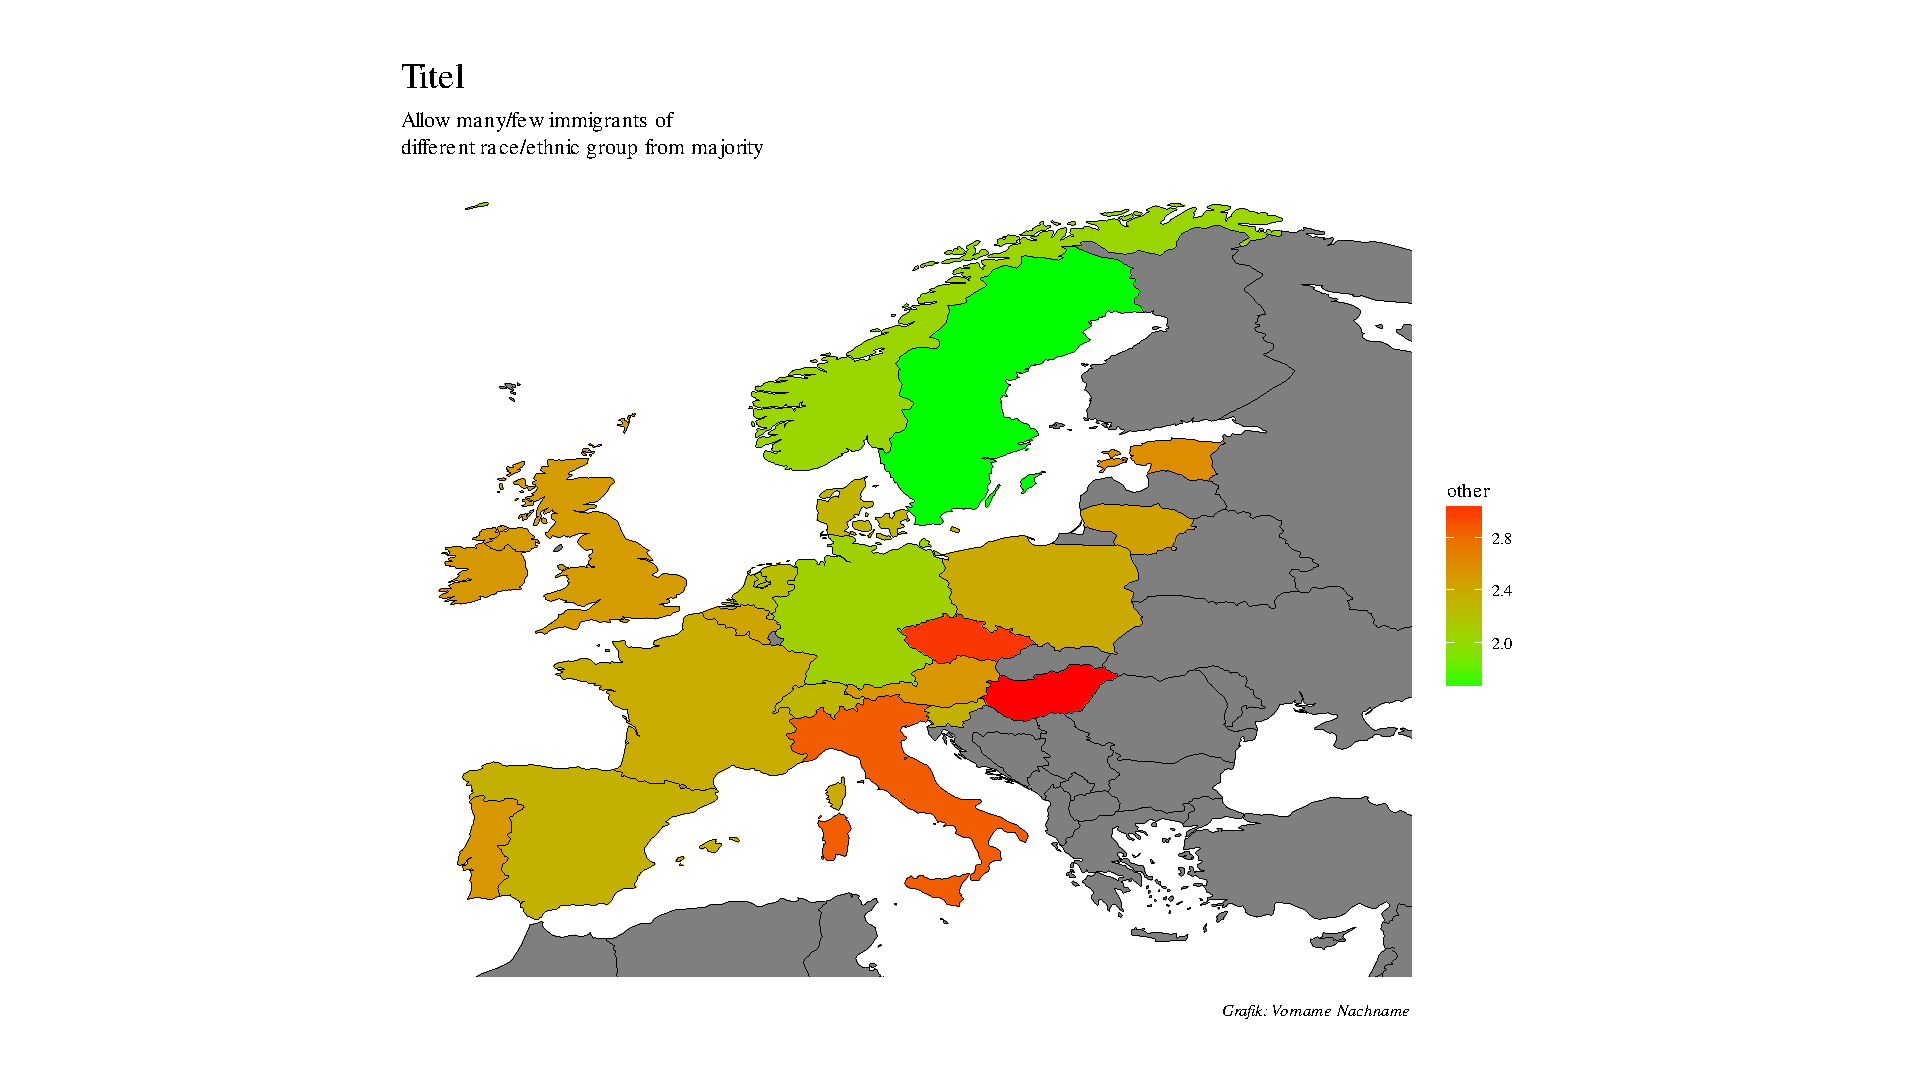
\includegraphics[width=0.75\textwidth]{results/figures/a3.pdf}
\end{figure}

\begin{table}
\begin{scriptsize}
%\input{tables/table1}
\end{scriptsize}
\caption{A table using stargazer}
\end{table}

\begin{table}
\begin{scriptsize}
%\input{tables/table2}
\end{scriptsize}
\caption{Another table using stargazer}
\end{table}

\newpage

\printbibliography
\end{document}